\hypertarget{agds_agdsPres}{}\section{Presentation}\label{agds_agdsPres}
The {\bfseries Ascii Graphic Database System (A\-G\-D\-S)} format is an ascii (text) version of the wellknown and industry standard G\-D\-S I\-I binary format. This format hierarchicaly represents geometric shapes, labels and other layout informations (see \href{http://en.wikipedia.org/wiki/GDSII}{\tt http\-://en.\-wikipedia.\-org/wiki/\-G\-D\-S\-I\-I} for more informations). \par
The ascii format has several advantages versus binary format\-:
\begin{DoxyItemize}
\item human readable,
\item easy to edit manually or with dedicated tools,
\item easy to search or grep into,
\item easy to compare and understand differences between two files,
\item easy to convert.
\end{DoxyItemize}

The conversion from Ascii G\-D\-S to binary G\-D\-S and vice versa can be done with {\bfseries Owl\-Vision G\-D\-S\-I\-I Viewer} available at \href{http://owlvision.org}{\tt http\-://owlvision.\-org}\par
Since it has been developped in java, it can be run on all platforms.\hypertarget{agds_agdsAutrhos}{}\subsection{Author}\label{agds_agdsAutrhos}
Damien Dupuis\-: damien.\-dupuis(at)lip6(.)fr\hypertarget{agds_agdsLimits}{}\subsection{Limitations}\label{agds_agdsLimits}
Currently the only supported shape in this driver is the rectangle.\hypertarget{agds_agdsDB}{}\section{Stand alone database structure}\label{agds_agdsDB}
The database conists in for simple objects \-:
\begin{DoxyItemize}
\item \hyperlink{class_a_g_d_s_1_1_library}{A\-G\-D\-S\-::\-Library} contains all A\-G\-D\-S library informations such as the name, the units used (user and physical) and the list of all Structures.
\item \hyperlink{class_a_g_d_s_1_1_structure}{A\-G\-D\-S\-::\-Structure} describes a G\-D\-S Structure with a name and a list of Elements.
\item \hyperlink{class_a_g_d_s_1_1_element}{A\-G\-D\-S\-::\-Element} is an abstract class from which derived the \hyperlink{class_a_g_d_s_1_1_rectangle}{A\-G\-D\-S\-::\-Rectangle}.
\item \hyperlink{class_a_g_d_s_1_1_rectangle}{A\-G\-D\-S\-::\-Rectangle} describes a rectangle element of a structure.
\end{DoxyItemize}\hypertarget{agds_agdsDriver}{}\subsection{Using the driver}\label{agds_agdsDriver}
To drive an A\-G\-D\-S file, user has to create one \hyperlink{class_a_g_d_s_1_1_library}{A\-G\-D\-S\-::\-Library} and add \hyperlink{class_a_g_d_s_1_1_structure}{A\-G\-D\-S\-::\-Structure} objects to it with the \hyperlink{class_a_g_d_s_1_1_library_a93d333a20154e0b688ff3ff213039171}{A\-G\-D\-S\-::\-Library\-::add\-Structure()} method. Each \hyperlink{class_a_g_d_s_1_1_structure}{A\-G\-D\-S\-::\-Structure} contains at least one \hyperlink{class_a_g_d_s_1_1_element}{A\-G\-D\-S\-::\-Element} added with \hyperlink{class_a_g_d_s_1_1_structure_a2dd203e6770f7d15d6f706867c919a60}{A\-G\-D\-S\-::\-Structure\-::add\-Element()} method.\par
All objects can be independently created as far as they are correctly added to their parent. \par
Once the library is completely specified, simply call the \hyperlink{class_a_g_d_s_1_1_library_a33b9d989b84857f46034085664ff3fa2}{A\-G\-D\-S\-::\-Library\-::write\-To\-File()} method to drive the database to file.\hypertarget{agds_agdsExamples}{}\section{Examples}\label{agds_agdsExamples}
As said is the global presentation, V\-L\-S\-I S\-A\-P\-D project provides C++ libraries and Python modules for each supported format. In this section we present two simple code examples to drive a A\-G\-D\-S file using C++ or Python. These two examples drive the same file {\ttfamily transistor.\-agds\-:} 
\begin{DoxyCodeInclude}
HEADER 5;
BGNLIB;
  LASTMOD \{10-06-11  14:02:15\};
  LASTACC \{10-06-11  14:02:15\};
LIBNAME myTestLib.DB;
UNITS;
  USERUNITS 0.001;
  PHYSUNITS 1.000000e-09;

BGNSTR;
  CREATION \{10-06-11  14:02:15\};
  LASTMOD  \{10-06-11  14:02:15\};
STRNAME Transistor;

BOUNDARY;
LAYER 17;
DATATYPE 0;
XY 5;
  X: 305;   Y: 150;
  X: 305;   Y: 830;
  X: 365;   Y: 830;
  X: 365;   Y: 150;
  X: 305;   Y: 150;
ENDEL;

BOUNDARY;
LAYER 6;
DATATYPE 0;
XY 5;
  X: 130;   Y: 290;
  X: 130;   Y: 690;
  X: 540;   Y: 690;
  X: 540;   Y: 290;
  X: 130;   Y: 290;
ENDEL;

ENDSTR;
ENDLIB;
\end{DoxyCodeInclude}


 
\begin{DoxyImage}
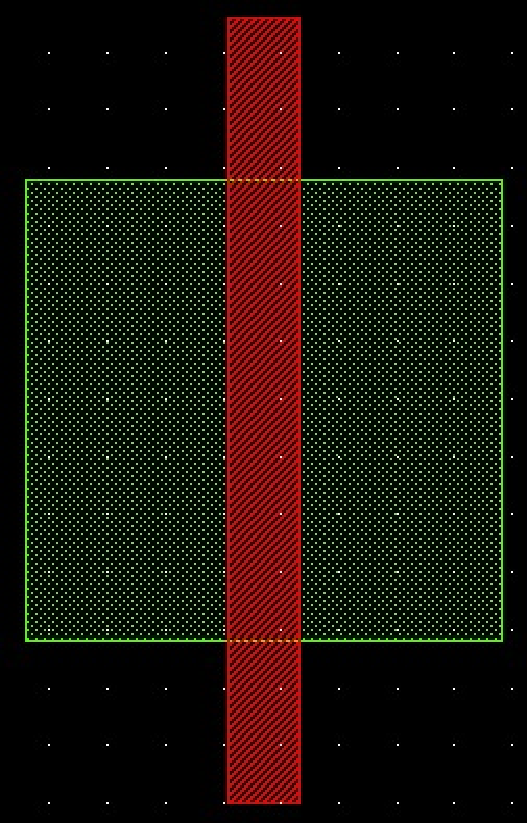
\includegraphics{transistorCif}
\caption{A\-G\-D\-S example layout width=.25}
\end{DoxyImage}
\hypertarget{agds_agdsC}{}\subsection{C++}\label{agds_agdsC}
Here is the C++ code ({\ttfamily drive\-Agds.\-cpp}) used to generate the transistor.\-agds file. (Source is available in examples directory). 
\begin{DoxyCodeInclude}
\textcolor{preprocessor}{#include <string>}
\textcolor{keyword}{using namespace }std;

\textcolor{preprocessor}{#include "vlsisapd/agds/Library.h"}
\textcolor{preprocessor}{#include "vlsisapd/agds/Structure.h"}
\textcolor{preprocessor}{#include "vlsisapd/agds/Rectangle.h"}

\textcolor{keywordtype}{int} main(\textcolor{keywordtype}{int} argc, \textcolor{keywordtype}{char} * argv[]) \{
    \hyperlink{class_a_g_d_s_1_1_library}{AGDS::Library}* lib = \textcolor{keyword}{new} \hyperlink{class_a_g_d_s_1_1_library}{AGDS::Library}(\textcolor{keywordtype}{string}(\textcolor{stringliteral}{"myTestLib"}));

    lib->\hyperlink{class_a_g_d_s_1_1_library_a0d0e972bb142f892c462bb8d7f04a50b}{setUserUnits}(0.001);
    lib->\hyperlink{class_a_g_d_s_1_1_library_a938acb6eb8d14aade9dba7331c75ff0a}{setPhysUnits}(1.0E-9);

    \hyperlink{class_a_g_d_s_1_1_rectangle}{AGDS::Rectangle}* poly   = \textcolor{keyword}{new} \hyperlink{class_a_g_d_s_1_1_rectangle}{AGDS::Rectangle}( 17, 305, 150, 365, 830 );
    \hyperlink{class_a_g_d_s_1_1_rectangle}{AGDS::Rectangle}* active = \textcolor{keyword}{new} \hyperlink{class_a_g_d_s_1_1_rectangle}{AGDS::Rectangle}(  6, 130, 290, 540, 690 );

    \hyperlink{class_a_g_d_s_1_1_structure}{AGDS::Structure}* str = \textcolor{keyword}{new} \hyperlink{class_a_g_d_s_1_1_structure}{AGDS::Structure}(\textcolor{stringliteral}{"Transistor"});

    str->\hyperlink{class_a_g_d_s_1_1_structure_a2dd203e6770f7d15d6f706867c919a60}{addElement}(poly);
    str->\hyperlink{class_a_g_d_s_1_1_structure_a2dd203e6770f7d15d6f706867c919a60}{addElement}(active);

    lib->\hyperlink{class_a_g_d_s_1_1_library_a93d333a20154e0b688ff3ff213039171}{addStructure}(str);

    lib->\hyperlink{class_a_g_d_s_1_1_library_a33b9d989b84857f46034085664ff3fa2}{writeToFile}(\textcolor{stringliteral}{"./transistor.agds"});
    
    \textcolor{keywordflow}{return} 0;
\}

\end{DoxyCodeInclude}


\begin{DoxyNote}{Note}
In order to compile this code, a C\-Make\-Lists.\-txt file is provided. User must set the \$\-V\-L\-S\-I\-S\-A\-P\-D\-\_\-\-T\-O\-P variable before running these commands in the directory containing the C\-Make\-Lists.\-txt file\-: 
\begin{DoxyCode}
%> mkdir build; cd build
%> cmake ..
%> make
\end{DoxyCode}

\end{DoxyNote}
\hypertarget{agds_agdsPython}{}\subsection{Python}\label{agds_agdsPython}
Here is the Python code ({\ttfamily drive\-Agds.\-py}) used to generate the transistor.\-agds file. (Source is available in examples directory). 
\begin{DoxyCodeInclude}
1 \textcolor{keyword}{import} AGDS
2 lib = \hyperlink{class_a_g_d_s_1_1_library}{AGDS.Library}(\textcolor{stringliteral}{"myTestLib"})
3 lib.setUserUnits(0.001)
4 lib.setPhysUnits(1.0e-9)
5 
6 active = \hyperlink{class_a_g_d_s_1_1_rectangle}{AGDS.Rectangle}( 6, 120, 290, 540, 690) \textcolor{comment}{# layer  6 corresponds to active}
7 poly   = \hyperlink{class_a_g_d_s_1_1_rectangle}{AGDS.Rectangle}(17, 305, 150, 365, 830) \textcolor{comment}{# layer 17 corresponds to polysilicium}
8 
9 str = \hyperlink{class_a_g_d_s_1_1_structure}{AGDS.Structure}(\textcolor{stringliteral}{"Transistor"})
10 str.addElement(active)
11 str.addElement(poly)
12 
13 lib.addStructure(str)
14 lib.writeToFile(\textcolor{stringliteral}{"./transistor.agds"})
\end{DoxyCodeInclude}


\begin{DoxyNote}{Note}
In order to run the {\ttfamily drive\-Agds.\-py} script, user must ensure that \$\-P\-Y\-T\-H\-O\-N\-P\-A\-T\-H variable points to the directory containing A\-G\-D\-S.\-so module. 
\end{DoxyNote}
